\documentclass[a4paper,12pt,twoside,openright]{report}

\usepackage[pdfborder={0 0 0}]{hyperref}    % turns references into hyperlinks
\usepackage[margin=25mm]{geometry}  % adjusts page layout
\usepackage{graphicx}  % allows inclusion of PDF, PNG and JPG images
\usepackage{verbatim}
\usepackage{pdfpages}  % to embed proposal at the end of the dissertation
\usepackage{textcomp}

\renewcommand{\baselinestretch}{1.1}    % adjust line spacing to make
% more readable

\begin{document}
	
	\bibliographystyle{plain}
	
	
	%%%%%%%%%%%%%%%%%%%%%%%%%%%%%%%%%%%%%%%%%%%%%%%%%%%%%%%%%%%%%%%%%%%%%%%%
	% Title
	
	
	\pagestyle{empty}
	
	\rightline{\LARGE \textbf{Peter Lotts}}
	
	\vspace*{60mm}
	\begin{center}
		\Huge
		\textbf{Adding network subsystem provenance collection to CADETS} \\[5mm]
		Computer Science Tripos -- Part II \\[5mm]
		Downing College \\[5mm]
		\today  % today's date
	\end{center}
	
	%%%%%%%%%%%%%%%%%%%%%%%%%%%%%%%%%%%%%%%%%%%%%%%%%%%%%%%%%%%%%%%%%%%%%%%%%%%%%%
	% Proforma, table of contents and list of figures
	
	\pagestyle{plain}
	
	\chapter*{Proforma}
	
	{\large
		\begin{tabular}{ll}
			Name:               & \bf Peter Lotts                       \\
			College:            & \bf Downing College                     \\
			Project Title:      & \bf Adding network subsystem provenance \\
								& \bf collection to CADETS \\
			Examination:        & \bf Computer Science Tripos -- Part II, 2018  \\
			Word Count:         & \bf tbc\footnotemark[1]  \\
			Project Originator: & Dr R.~Sohan                    \\
			Supervisor:         & Dr G.~Jenkinson                    \\ 
		\end{tabular}
	}
	\footnotetext[1]{This word count was computed at [date]	by the provided online tool at \texttt{URL}
	}
	\stepcounter{footnote}
	
	
	\section*{Original Aims of the Project}
	
	To provide additional metadata collection tools for network packets to the Computer Laboratory's existing CADETS project. This will be provided by tracking individual packets as they flow through the network stack of the FreeBSD\footnote{\texttt{http://www.freebsd.org/}} kernel, and making information regarding memory locations used and the time taken by each layer to process a given packet available to DTrace\footnote{\texttt{http://dtrace.org/}}. DTrace is a generic Dynamic Tracing framework which is the primary data collection tool used by the CADETS project to bring kernel data into userspace for analysis. The performance impact of the project on network packet delivery is to be evaluated.
	
	
	\section*{Work Completed}
	
	\textit{What we actually did.}
	
	\section*{Special Difficulties}
	
	None. [We hope!!]
	
	\newpage
	\section*{Declaration Of Originality}
	
	I, Peter Lotts of Downing College, being a candidate for Part II of
	the Computer Science Tripos, hereby declare
	that this dissertation and the work described in it are my own work,
	unaided except as may be specified below, and that the dissertation
	does not contain material that has already been used to any substantial
	extent for a comparable purpose.
	
	\bigskip
	\leftline{Signed [signature]}
	
	\medskip
	\leftline{Date [date]}
	
	\tableofcontents
	
	\listoffigures
	
%	\newpage
%	\section*{Acknowledgements}
	
%	This document owes much to an earlier version written by Simon Moore
%	\cite{Moore95}.  His help, encouragement and advice was greatly 
%	appreciated.
	
	%%%%%%%%%%%%%%%%%%%%%%%%%%%%%%%%%%%%%%%%%%%%%%%%%%%%%%%%%%%%%%%%%%%%%%%
	% now for the chapters
	
	\pagestyle{headings}
	
	\chapter{Introduction}
	
	\section{Background [Use Case?]}
	
	Nowadays, most cyberattacks from nation state actors do not take on the traditional form of a piece	of malware which tries to find a store of sensitive data and dump it back to the attacker as quickly as	possible before system administrators have time to intervene. Instead, these attacks slowly 	infiltrate the target system, hiding out of sight and learning the use patterns of normal users. They then exploit this knowledge to slowly make horizontal transfers within the target enterprise’s internal	network, and extract sensitive data from databases in such a way that the access is hard to	distinguish from normal access. Such an attack is called an Advanced Persistent Threat (APT), and can go on for months or years without system administrators realising. Eventually, it is likely that the malware will make a mistake and trigger an indicator of compromise to be observed by administrators, but by then it is difficult to tell when and how the malware entered the system, and what data it has seen. This can make impact assessments, as well as efforts to prevent a similar attack in future, very difficult.
	
	The Computer Laboratory has a project which is trying to combat this by building CADETS, a Causal, Adaptive, Distributed, and Efficient Tracing System, on top of the FreeBSD operating system. The system is being built to track the provenance of data by collecting metadata from computers all over the network about what processes act on what data and when. This metadata is then collected in a distributed database, where it can be analysed to trace data flows throughout the computer system. This should allow analysts to trace malware back to possible entry times and methods, which they can then analyse further.
	
	This project will add support for collecting metadata on network packets as they flow through the kernel	network stack. The data collected will allow users of CADETS to seek out suspicious activity which may be being used to attack a system, and will be able to provide a list of locations in kernel memory where packet data were stored. The latter allows a rapid impact assessment to be produced if a system administrator is able to determine that some malicious code had access to a particular set of kernel memory addresses, as CADETS will let the administrator infer what data may have been leaked.
	
	\section{The Network Stack}
	
	Provide a brief explanation of the concept of the network stack up to the socket API, layering, fragmentation etc.
	
	\section{Tracing as a Security Tool}
	
	Discuss why CADETS is useful, point out that we can't generally assume the security of a system to be perfectly watertight (Meltdown/Spectre), and the need for something to pick up the pieces later.
	
	\section{Similar Work}
	
	Just need to mention Resourceful? - I haven't used it so far, is it even relevant?
	
	\section{Overall design}
	
	The project is to assign uniquely identifying tags to each packet as it flows through the network stack, noting that packet fragmentation/reassembly will make this more difficult. This will then allow DTrace tracepoints to read the tag on each packet when an interesting operation (broadly speaking, a memory allocation) is performed on it. From here, scripts written in DTrace's D language will be able to forward information to the CADETS userspace application for processing.
	
%%%%% Template version - kept for useful formatting constructs	
	
	\section{Overview of the files}
	
	This document consists of the following files:
	
	\begin{itemize}
		\item \texttt{makefile} --- The makefile for the dissertation and
		Project Proposal
		\item \texttt{diss.tex} --- The dissertation
		\item \texttt{proposal.tex}  --- The project proposal 
		\item \texttt{figs} -- A directory containing diagrams and pictures
		\item \texttt{refs.bib} --- The bibliography database
	\end{itemize}
	
	\section{Building the document}
	
	This document was produced using \LaTeXe which is based upon
	\LaTeX\cite{Lamport86}.  To build the document you first need to
	generate \texttt{diss.aux} which, amongst other things, contains the
	references used.  This if done by executing the command:
	
	\texttt{pdflatex diss}
	
	\noindent
	Then the bibliography can be generated from \texttt{refs.bib} using:
	
	\texttt{bibtex diss}
	
	\noindent
	Finally, to ensure all the page numbering is correct run \texttt{pdflatex}
	on \texttt{diss.tex} until the \texttt{.aux} files do not change.  This
	usually takes 2 more runs.
	
	\subsection{The makefile}
	
	To simplify the calls to \texttt{pdflatex} and \texttt{bibtex}, 
	a makefile has been provided, see Appendix~\ref{makefile}. 
	It provides the following facilities:
	
	\begin{description}
		
		\item\texttt{make} \\
		Display help information.
		
		\item\texttt{make proposal.pdf} \\
		Format the proposal document as a PDF.
		
		\item\texttt{make view-proposal} \\
		Run \texttt{make proposal.pdf} and then display it with a Linux PDF viewer
		(preferably ``okular'', if that is not available fall back to ``evince'').
		
		\item\texttt{make diss.pdf} \\
		Format the dissertation document as a PDF.
		
		\item\texttt{make count} \\
		Display an estimate of the word count.
		
		\item\texttt{make all} \\
		Construct \texttt{proposal.pdf} and \texttt{diss.pdf}.
		
		\item\texttt{make pub} \\ Make \texttt{diss.pdf}
		and place it in my \texttt{public\_html} directory.
		
		\item\texttt{make clean} \\ Delete all intermediate files except the
		source files and the resulting PDFs. All these deleted files can
		be reconstructed by typing \texttt{make all}.
		
	\end{description}
	
	
	\section{Counting words}
	
	An approximate word count of the body of the dissertation may be
	obtained using:
	
	\texttt{wc diss.tex}
	
	\noindent
	Alternatively, try something like:
	
	\verb/detex diss.tex | tr -cd '0-9A-Z a-z\n' | wc -w/
	
	
	\chapter{Preparation}
	

	
	\chapter{Implementation}
	
	\section{Verbatim text}
	
	Verbatim text can be included using \verb|\begin{verbatim}| and
	\verb|\end{verbatim}|. I normally use a slightly smaller font and
	often squeeze the lines a little closer together, as in:
	
	{\renewcommand{\baselinestretch}{0.8}\small
		\begin{verbatim}
		GET "libhdr"
		
		GLOBAL { count:200; all  }
		
		LET try(ld, row, rd) BE TEST row=all
		THEN count := count + 1
		ELSE { LET poss = all & ~(ld | row | rd)
		UNTIL poss=0 DO
		{ LET p = poss & -poss
		poss := poss - p
		try(ld+p << 1, row+p, rd+p >> 1)
		}
		}
		LET start() = VALOF
		{ all := 1
		FOR i = 1 TO 12 DO
		{ count := 0
		try(0, 0, 0)
		writef("Number of solutions to %i2-queens is %i5*n", i, count)
		all := 2*all + 1
		}
		RESULTIS 0
		}
		\end{verbatim}
	}
	
	\section{Tables}
	
	\begin{samepage}
		Here is a simple example\footnote{A footnote} of a table.
		
		\begin{center}
			\begin{tabular}{l|c|r}
				Left      & Centred & Right \\
				Justified &         & Justified \\[3mm]
				%\hline\\%[-2mm]
				First     & A       & XXX \\
				Second    & AA      & XX  \\
				Last      & AAA     & X   \\
			\end{tabular}
		\end{center}
		
		\noindent
		There is another example table in the proforma.
	\end{samepage}
	
	\section{Simple diagrams}
	
	Simple diagrams can be written directly in \LaTeX.  For example, see
	figure~\ref{latexpic1} on page~\pageref{latexpic1} and see
	figure~\ref{latexpic2} on page~\pageref{latexpic2}.
	
	\begin{figure}
		\setlength{\unitlength}{1mm}
		\begin{center}
			\begin{picture}(125,100)
			\put(0,80){\framebox(50,10){AAA}}
			\put(0,60){\framebox(50,10){BBB}}
			\put(0,40){\framebox(50,10){CCC}}
			\put(0,20){\framebox(50,10){DDD}}
			\put(0,00){\framebox(50,10){EEE}}
			
			\put(75,80){\framebox(50,10){XXX}}
			\put(75,60){\framebox(50,10){YYY}}
			\put(75,40){\framebox(50,10){ZZZ}}
			
			\put(25,80){\vector(0,-1){10}}
			\put(25,60){\vector(0,-1){10}}
			\put(25,50){\vector(0,1){10}}
			\put(25,40){\vector(0,-1){10}}
			\put(25,20){\vector(0,-1){10}}
			
			\put(100,80){\vector(0,-1){10}}
			\put(100,70){\vector(0,1){10}}
			\put(100,60){\vector(0,-1){10}}
			\put(100,50){\vector(0,1){10}}
			
			\put(50,65){\vector(1,0){25}}
			\put(75,65){\vector(-1,0){25}}
			\end{picture}
		\end{center}
		\caption{A picture composed of boxes and vectors.}
		\label{latexpic1}
	\end{figure}
	
	\begin{figure}
		\setlength{\unitlength}{1mm}
		\begin{center}
			
			\begin{picture}(100,70)
			\put(47,65){\circle{10}}
			\put(45,64){abc}
			
			\put(37,45){\circle{10}}
			\put(37,51){\line(1,1){7}}
			\put(35,44){def}
			
			\put(57,25){\circle{10}}
			\put(57,31){\line(-1,3){9}}
			\put(57,31){\line(-3,2){15}}
			\put(55,24){ghi}
			
			\put(32,0){\framebox(10,10){A}}
			\put(52,0){\framebox(10,10){B}}
			\put(37,12){\line(0,1){26}}
			\put(37,12){\line(2,1){15}}
			\put(57,12){\line(0,2){6}}
			\end{picture}
			
		\end{center}
		\caption{A diagram composed of circles, lines and boxes.}
		\label{latexpic2}
	\end{figure}
	
	
	
	\section{Adding more complicated graphics}
	
	The use of \LaTeX\ format can be tedious and it is often better to use
	encapsulated postscript (EPS) or PDF to represent complicated graphics.
	Figure~\ref{epsfig} and~\ref{xfig} on page \pageref{xfig} are
	examples. The second figure was drawn using \texttt{xfig} and exported in
	{\tt.eps} format. This is my recommended way of drawing all diagrams.
	
	
	\begin{figure}[tbh]
%		\centerline{\includegraphics{figs/cuarms.pdf}}
		\caption{Example figure using encapsulated postscript}
		\label{epsfig}
	\end{figure}
	
	\begin{figure}[tbh]
		\vspace{4in}
		\caption{Example figure where a picture can be pasted in}
		\label{pastedfig}
	\end{figure}
	
	
	\begin{figure}[tbh]
%		\centerline{\includegraphics{figs/diagram.pdf}}
		\caption{Example diagram drawn using \texttt{xfig}}
		\label{xfig}
	\end{figure}
	
	
	\chapter{Evaluation}
	
	\section{Printing and binding}
	
	Use a ``duplex'' laser printer that can print on both sides to print
	two copies of your dissertation. Then bind them, for example using the
	comb binder in the Computer Laboratory Library.
	
	\section{Further information}
	
	See the Unix Tools notes at
	
	\url{http://www.cl.cam.ac.uk/teaching/current-1/UnixTools/materials.html}
	
	
	\chapter{Conclusion}
	
	I hope that this rough guide to writing a dissertation is \LaTeX\ has
	been helpful and saved you time.
	
	
	%%%%%%%%%%%%%%%%%%%%%%%%%%%%%%%%%%%%%%%%%%%%%%%%%%%%%%%%%%%%%%%%%%%%%
	% the bibliography
	\addcontentsline{toc}{chapter}{Bibliography}
	\bibliography{refs}
	
	%%%%%%%%%%%%%%%%%%%%%%%%%%%%%%%%%%%%%%%%%%%%%%%%%%%%%%%%%%%%%%%%%%%%%
	% the appendices
	\appendix
	
	
	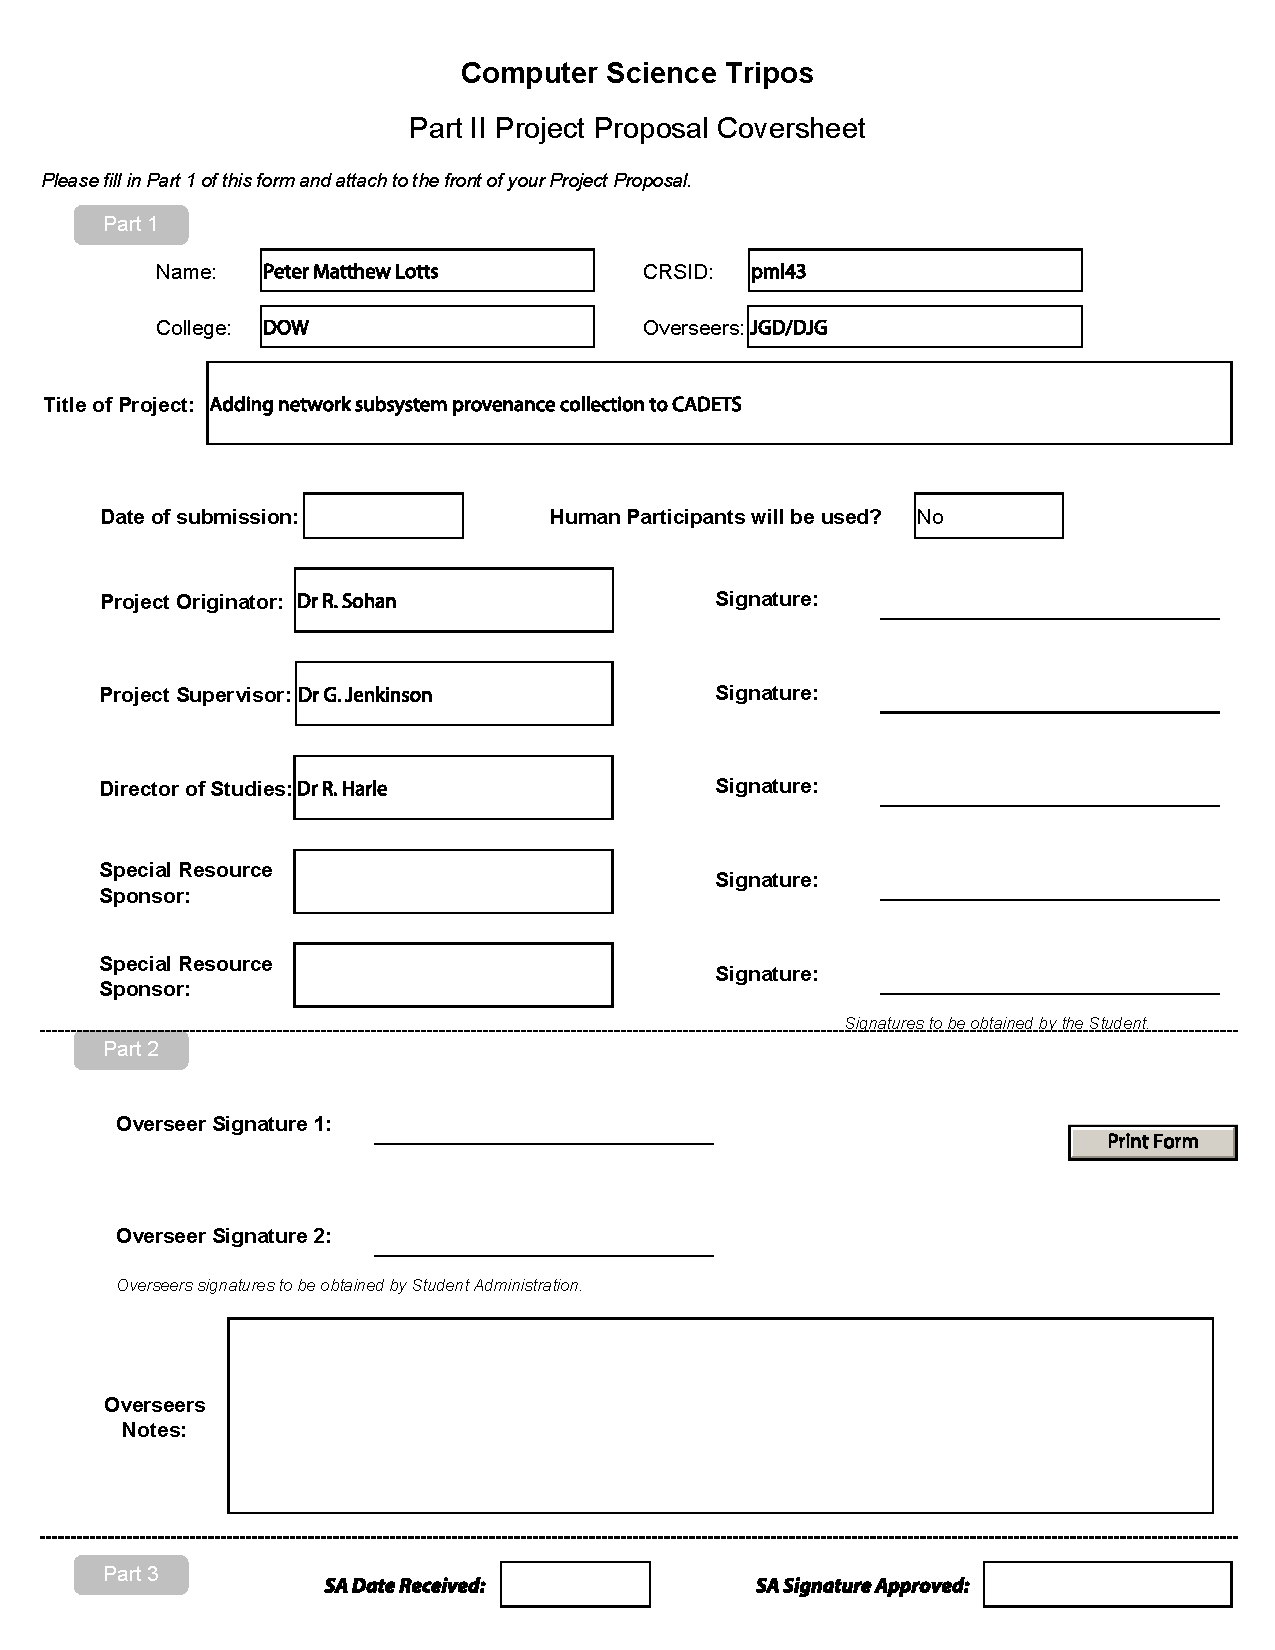
\includepdf{include/Project-Proposal-Cover-Sheet.pdf}
	\includepdf[pages={2-}]{include/Project-Proposal.pdf}
	
	
\end{document}
